\chapter{Related work}

\section{Image forgery}

When dealing with a digital image, it is quite common to wonder if it is original or has been counterfeited in some way. Images and videos have become the main information carriers in the digital era and used to store real world events, but  they are very easy to manipulate because of the availability of the powerful editing software and sophisticated digital cameras.

The contexts where doctored pictures could be involved are very disparate; they could be used in a tabloid or in an advertising poster or included in a journalistic report but also in a court of law where digital (sometimes printed) images are presented as crucial evidences for a trial in order to influence the final judgement. So, especially in the last case, reliably assessing image integrity becomes of fundamental importance. 

\emph{Image forensics} specifically deals with such issues by studying and developing technological tools which generally permit determining, by only analyzing a digital photograph (i.e., its pixels), if that asset has been manipulated or even which could have been the adopted acquisition device (such an issue is not relevant to the topic of the present paper). Moreover, if it has been established that something has been altered, it could be important to understand in which part of the image itself such a modification occurred, for instance, if a person or a specific object has been covered, if an area of the image has been cloned, if something (i.e., a face or a weapon) has been copied from another different image, or, even more, if a mixture of these processes has been carried out. 

\section{Image forgery detection techniques}

To verify the authenticity of a picture many techniques have been identified that can be categorized into active (intrusive) and blind (non-intrusive).

Operative techniques involve a phase of preprocessing the image itself at the time of its creation in order to include some additional information that will be used during the analysis phase. An example of operative technique is the watermarking.

Passive techniques analyze the content of the image using various statistics or semantic content in order to identify inconsistencies of some kind. This approach does not alter the contents of the image.
There is a general technique, suitable to capture all kinds of inconsistencies present in an image, but each different method specialises in the identification of a particular type.

\section{Image splicing}

Image splicing is a very common type of infringement which basically consists in copying a region of a given image to another, thus creating a composition of two different pictures together.

\begin{figure}
  \centering
    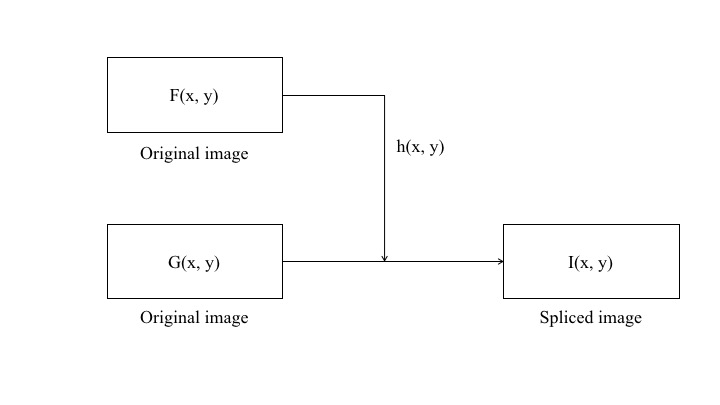
\includegraphics[width=0.8\textwidth]{imagesplicing}
    \caption{Image splicing process}
\end{figure}

Image splicing consists of using parts of two or more images to compose a new image that never took place in space and time. 

This composition process includes all the necessary operations (such as brightness and contrast adjustment, affine transformations, color changes, etc.) to construct realist images able to deceive viewer. In this process, normally, we refer to the parts coming from other images as aliens and the image receiving the other parts as host.

One of the common studied case is image composition involving people are very popular and are employed with very different objectives. 

\subsection{Some famous cases}

Photography has lost its innocence since the early days of his birth. In fact already in 1860, only a few decades after Niépce created the first photo, the first manipulated photographs were identified in 1826. With the advent of digital cameras, camcorders and sophisticated photo editing software, digital image manipulation is becoming more common. 

\paragraph{O.J. Simpson - June 1994}

This altered photography O.J. Simpson appeared on the cover of the magazine Time Magazine, soon after his arrest for murder. 

\begin{wrapfigure}{r}{0.5\textwidth}
  \begin{center}
    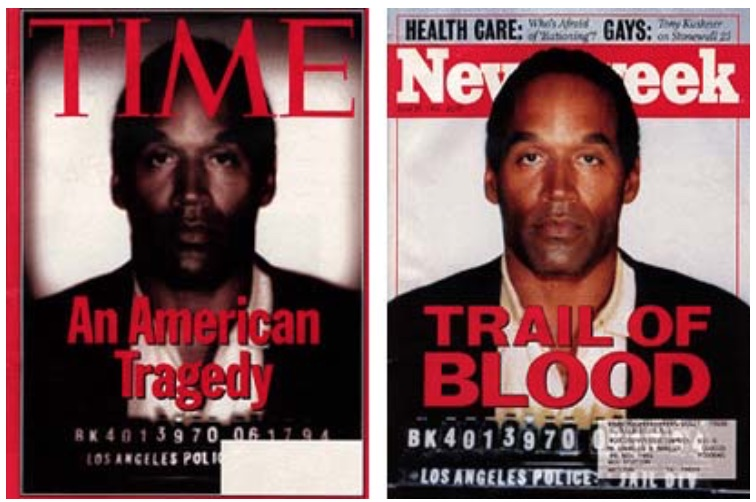
\includegraphics[width=0.48\textwidth]{ojsimpson}
  \end{center}
  \caption{The Time Magazine and O.J. Simpson}
  \vspace{-1cm}
\end{wrapfigure}

In fact, the photograph was altered compared to the original image that has appeared on the cover of Newsweek magazine. Time magazine was accused of manipulation of the photography in order to make darker and menacing figure of Simpson.

\paragraph{Iraq - April 2003}

This composition of a British soldier in Basra, which keeps pointing toward a civilian Iraqi gesticulates covered, she appeared on the cover of the Los Angeles Times, immediately after the invasion of Iraq. 

\begin{wrapfigure}{l}{0.5\textwidth}
  \begin{center}
    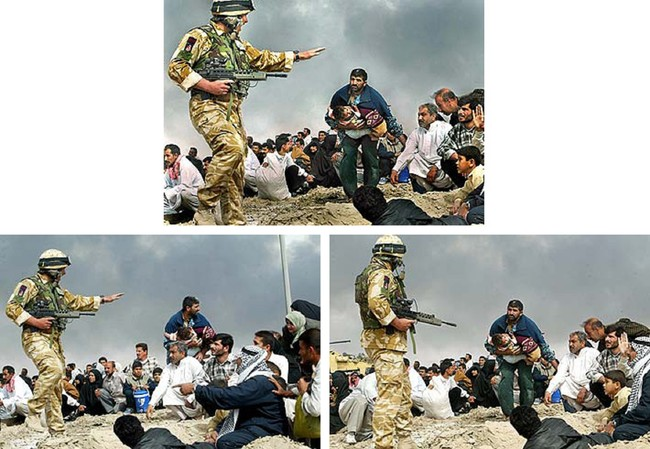
\includegraphics[width=0.48\textwidth]{iraq}
  \end{center}
  \caption{An example of image composition}
\end{wrapfigure}

Brian Walski, a staff photographer for the Los Angeles Times and a veteran of the news with thirty years of experience, was summarily fired from his publisher for their merged two of his shots in order to improve the composition.

\paragraph{George W. Bush - March 2004}

This image, taken from promo released for the election campaign of George w. Bush, outlined a packed audience of soldiers as a backdrop to a child who was flying the American flag. This image was digitally souped-up, using a crude copy and paste, removing Bush from the podium. 

\begin{wrapfigure}{r}{0.5\textwidth}
  \begin{center}
    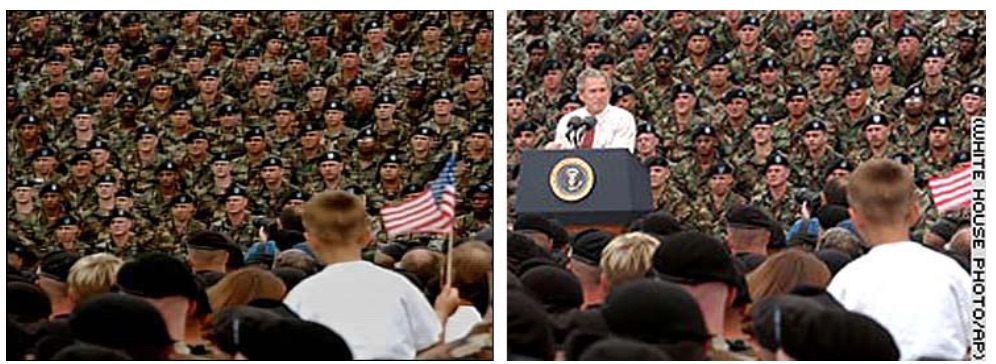
\includegraphics[width=0.48\textwidth]{bush}
  \end{center}
  \caption{An example of image composition}
\end{wrapfigure}


After admitting the tampering with the staff of the television station edited and sent to Bush promo with the original photo.

Cases such as this show how present image composition is in our daily lives. Unfortunately, it also decreases our trust on images and highlights the need for developing methods for recovering back such confidence.

\section{Methods based on light inconsistencies}

Methods for detecting image composition have become actual and powerful tools in the forensic analysis process. Different types of methods have been proposed for detecting image composition. Methods based on inconsistencies in compatibility metrics, JPEG compression features and perspective constraints are just a few examples of inconsistencies explored to detect forgeries.

After studying and analyzing the advantages and drawbacks of different types of methods for detecting image composition, this work herein relies on the research hypothesis that image illumination inconsistencies are strong and powerful evidence of image composition.

This hypothesis has already been used by some researchers in the literature whose work will be detailed in the next chapter, and it is specially useful for detecting image composition because, even for expert counterfeiters, a perfect illumination match is extremely hard to achieve. Also, there are some experiments that show how difficult is for humans perceive image illumination inconsistencies.

We can divide methods that explore illumination inconsistencies into three main groups of methods:
\begin{enumerate}
\item methods based on inconsistencies in the \textbf{light setting}: this group of methods encloses approaches that look for inconsistencies in the light position and in models that aim at reconstructing the scene illumination conditions.
\item methods based on inconsistencies in the \textbf{shadows}: this group of methods encloses approaches that look for inconsistencies in the scene illumination using telltales derived from shadows.
\item methods based on inconsistencies in \textbf{light color}: this group of methods encloses approaches that look for inconsistencies in the color of illuminants present in the scene.
\end{enumerate}


\subsection{Inconsistencies in the light setting}

Johnson and Farid\cite{Johnson:2005:EDF:1073170.1073171} proposed an approach based on illumination inconsistencies, looking for chromaticity aberrations as an indicator of image forgery. They analyzed the light source direction from different objects in the same image trying to detect traces of tampering. The authors start by imposing different constraints for the problem:

\begin{enumerate}
\item All the analyzed objects have \emph{Lambertian surface}\footnote{A Lambertian surface for reflection is a surface that appears uniformly bright from all directions of view and reflects the entire incident light. Lambertian reflectance is the property exhibited by an ideal matte or diffusely reflecting surface.}.
\item The surface reflectance is constant.
\item The object surface is illuminated by an infinitely distant light source.
\end{enumerate}

Using RGB images, the authors assume that the chromaticity deviation is constant (and dependent on each channel wavelength) for all color channels and create a model, based on image statistical properties, of how the ray light should split for each color channel. Given this premise and using the green channel as reference, the authors estimate deviations between the red and green channels and between the blue and green channels for selected parts of the image. Inconsistencies on this split pattern are used as telltales to detect forgeries. 

A drawback of this method is that chromaticity deviation depends on the camera lens used to take the picture. 

\subsection{Inconsistencies in the shadows}

Another set of methods is based on inconsistencies on the shadows in the image.
 
Zhang and Wang \cite{zhang2009detecting} proposed an approach that utilizes the planar homology\cite{springer1964geometry}, which models the relationship of shadows in an image for discovering forgeries.

Based on this model, the authors proposed to construct two geometric constraints: the first one is based on the relationship of connecting lines. A connecting line is a line that connects some object point with its shadow. According to planar homology, all of these connecting lines intersect in a vanishing point. 

\begin{figure}
  \centering
    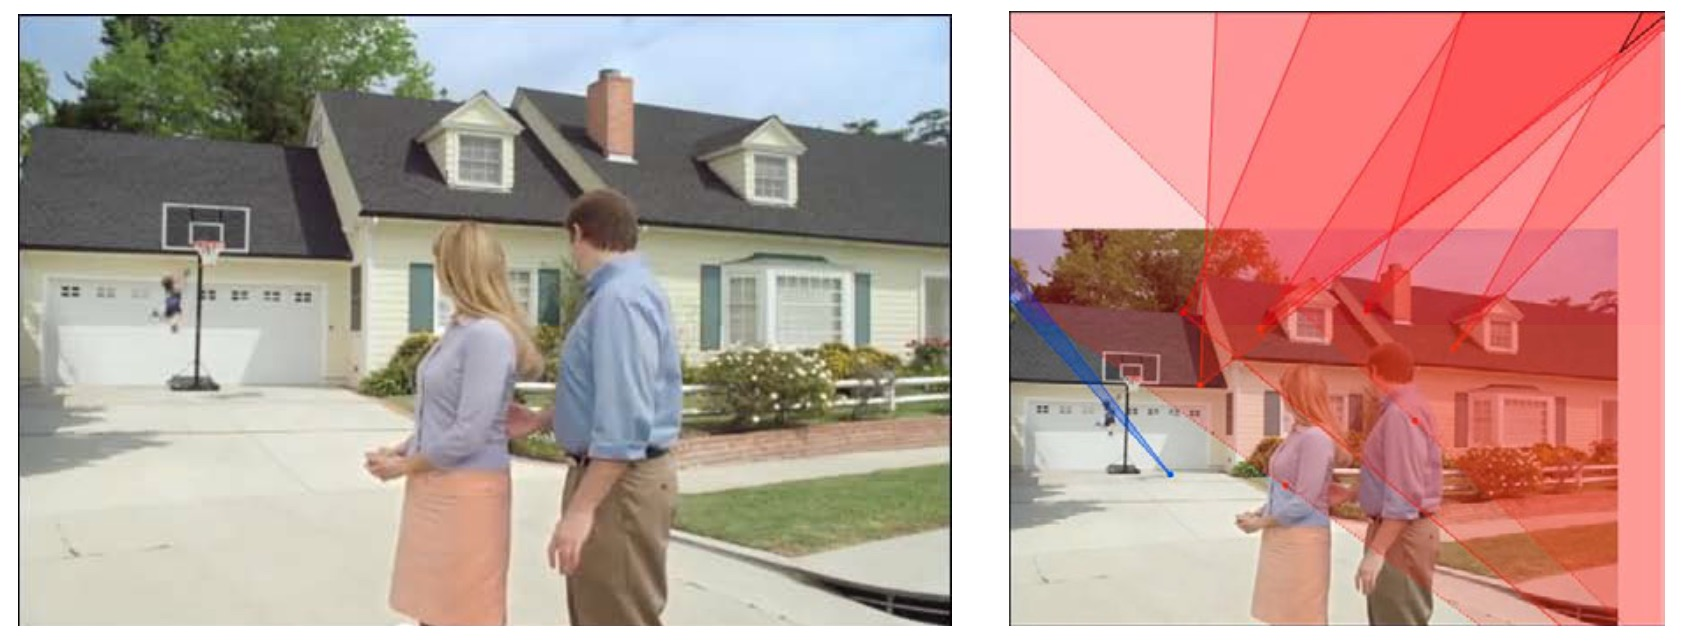
\includegraphics[width=0.8\textwidth]{shadows_inconsistencies}
    \caption{Original image (left) and the extracted shadows constraints (right)}
    \label{shadows_inconsistencies}
\end{figure}

The second constraint is based on the ratio of these connecting lines. In addition, the authors also proposed to explore the changing ratio along the normal direction of the shadow boundaries. 

Geometric and shadow photometric constraints together are used to detect image compositions. However, in spite of being a good initial step in forensic shadow analysis, the major drawback of the method is that it only works with images containing casting shadows, a very restricted scenario.

\subsection{Inconsistencies in light color}

The last group of methods investigate the presence, or not, of composition operations in digital images using color inconsistencies.

Gholap and Bora\cite{gholap2008illuminant} pioneered this approach using the \emph{illuminant colors}. For that, the authors used a \emph{dichromatic reflection model} proposed by Tominaga and Wandell\cite{tominaga1989standard}, which assumes a single light source to estimate illuminant colors from images.

\begin{wrapfigure}{l}{0.5\textwidth}
  \begin{center}
    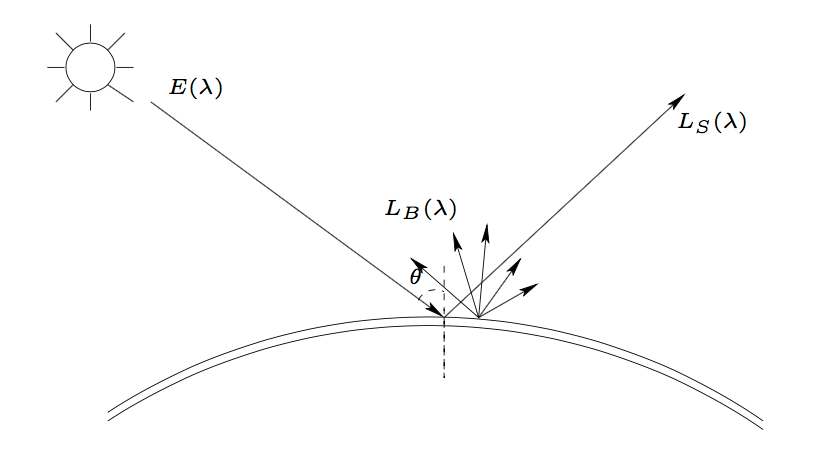
\includegraphics[width=0.48\textwidth]{dichromatic_reflection_model}
  \end{center}
  \label{dichromatic_reflection_model}
  \caption{The dichromatic reflection model}
\end{wrapfigure}


According to this model, reflection of any non-homogeneous materials may be modelled as additive mixture of two components, diffused reflection and surface reflection as shown in Fig. \ref{dichromatic_reflection_model}.

Considering an object point illuminated by a light source, the reflected ray consists of diffuse reflection $L_B (\lambda)$ and surface reflection $L_S (\lambda)$. The reflected light $L(\Theta, \lambda)$ can be written as:

\begin{equation} \label{eq:dichromaticmodel}
L(\Theta, \lambda) = m_S(\Theta) L_S(\lambda) + m_B(\Theta) L_B(\lambda)
\end{equation}

where $m_S(\Theta)$ and $m_B(\Theta)$ are geometrical factors and $\Theta$ the angle of the incident light. This equation can be rewritten in terms of RGB sensors in matrix form.

The two vectors $L_B(\lambda)$ and $L_S(\lambda)$ span the two dimensional plane called \emph{dichromatic plane}.

Dichromatic planes can also be estimated using principal component analysis (PCA) from each specular highlight region of an image. By applying a \emph{Singular Value Decomposition (SVD)} on the RGB matrix extracted from highlighted regions, the authors extract the eigenvectors associated with the two most significant eigenvalues to construct the \emph{dichromatic plane}. This plane is then mapped onto a straight line, named dichromatic line, in normalized \emph{r-g-chromaticity} space. 

For distinct objects illuminated by the same light source, the intersection point produced by their dichromatic line intersection represents the illuminant color. If the image has more than one illuminant, it will present more than one intersection point, which is not expected to happen in pristine (non-forged images). This method represented the first important step toward forgery detection using illuminant colors, but has some limitations such as the need of well defined specular highlight regions for estimating the illuminants.

Following Gholap and Bora’s work, Riess and Angelopoulou\cite{riess2010scene} used an extension of the \emph{Inverse-Intensity Chromaticity Space}, originally proposed by Tan et al.\cite{tan2004color}, to estimate illuminants locally from different parts of an image for detecting forgeries.

In addiction, Wu and Fang\cite{wu2011image} proposed a new way to detect forgeries using illuminant colors. Their method divides a color image into overlapping blocks estimating the illuminant color for each block. To estimate the illuminant color, the authors proposed to use the algorithms Gray-World, Gray-Shadow and Gray-Edge \cite{van2007edge}.

These approaches will be better explained in the next section due their importance for this proposed method.

\section{Illuminant color estimation}


The color of an object observed in an image depends both on its intrinsic color and the color of light source i.e., the illuminant. 

It is important to keep in mind that even the same light source can generate different illuminants. The illuminant formed by the sun, for example, varies in its appearance during the day and time of year as well as with the weather. We only capture the same illuminant, measuring the sunlight at the same place at the same time.

We can explore illuminants in forensics to check the consistency of similar objects in a scene. If two objects with very similar color stimuli (e.g., human skin) depict inconsistent appearance (different illuminants), it means they might have undergone different illumination conditions hinting at a possible image composition. On the other hand, if we have a photograph with two people and the color appearance on the faces of such people are consistent, it is likely they have undergone similar lighting conditions.

Riess and Angelopoulou\cite{riess2010scene} pioneered the approach of using a color-based method that investigates illuminant colors to detect forgeries in forensic scenario. In their work illuminant colors are estimated locally, effectively decomposing the scene in a map of differently illuminated regions. Inconsistencies in such a map suggest possible image tampering.

The method can be divided into four steps:

\begin{enumerate}
\item Image segmentation. The image is segmented into regions, called \emph{superpixels}, of approximately the same object color. Each superpixel follows must be:
\begin{enumerate}
\item Directly illuminated by the same light source.
\item Compliant with the \emph{dichromatic reflectance model}\cite{tan2004color}.
\end{enumerate}
\item Manual user selection of superpixels under investigation.
\item Local illuminant color estimation for each superpixel (both for segmented superpixels and user selected regions).
\item Reference illuminant selection (manual) and \emph{distance map} evaluation. The distance map is the base for an expert analysis for forgery detection.
\end{enumerate}

\begin{figure}
  \centering
    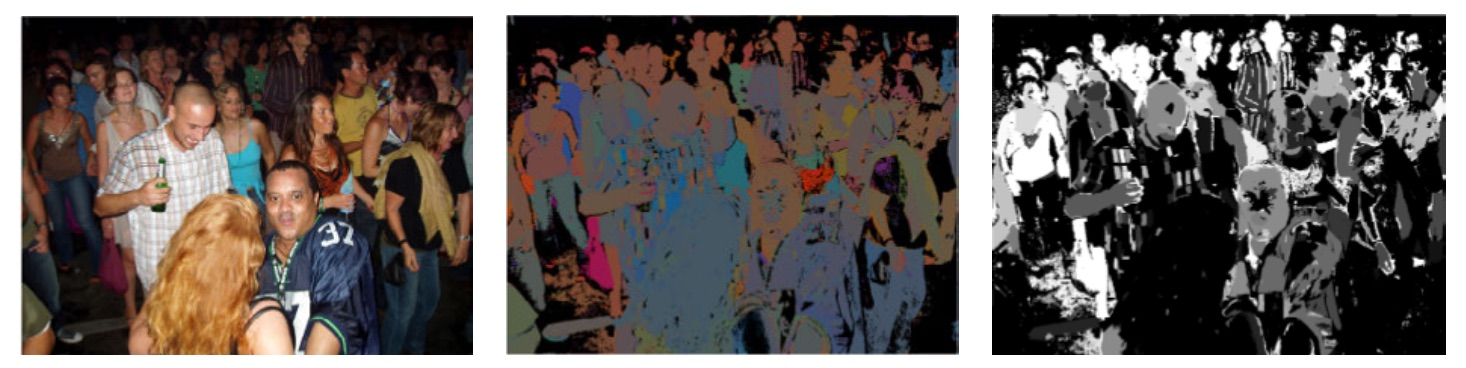
\includegraphics[width=0.95\textwidth]{illuminant_maps}
    \caption{An example of a generated distance map using Riess and Angelopoulou\cite{riess2010scene} approach. From left to right: (a) the original image, (b) \emph{illuminant map}, (c) generated distance map}
    \label{illuminant_maps}
\end{figure}

The final decision of this approach is delegated to an expert and not to the algorithm itself.

\subsection{Illuminant maps}


\subsubsection{Generalized Greyworld estimation}

The starting point is the \emph{gray world assumption}, proposed by Buchsbaum\cite{Buchsbaum19801}. In its simplest version, it is assumed that information in the average of each channel of the image is the representative gray level.

Let $f(x) = (\Gamma_R(x), \Gamma_G(x), \Gamma_B(x))^T$ the RGB color of a pixel at position $x$ and $\Gamma_i(x)$ the intensity of that pixel in the $i$-th channel. In their paper, Van de Weijer et al. assumes that the diffuse reflection id diffuse and that the camera response is linear. It is also assumed that the scene is illuminated by a single light source.

The RGB color $f(x)$ can also be rewritten as

\begin{equation}
f(x) = \int_{\omega} e(\beta, x) s(\beta, x) c(\beta) d\beta
\end{equation}

where $\omega$ is the visible light spectrum, $\beta$ is the light wavelenght, $e(\beta, x)$ is the illuminant spectrum, $s(\beta, x)$ is the surface reflectance of an object and $c(\beta)$ is the color sensitivities of the camera for each channel.

As an alternative to the gray-world hypothesis, Van de Weijer et al.\cite{van2007edge} proposed the \emph{gray-edge hypothesis}: the average of the reflectance differences in a scene is achromatic.

This idea load to a framework for low-level based illuminant estimation, called \emph{Generalized Grayworld}.

\begin{equation}\label{eq:ggeframework}
\left( \int 	\left | \frac{\delta^n f^{\sigma}(x)}{\delta x^{n}} \right |^{p} dx \right)^{\frac{1}{p}} = k e ^{n, p, \sigma}
\end{equation}

where $k$ denotes a scaling factor, $|\cdot|$ the norm operand, $\delta$ the differential operator and $f^{\sigma}(x)$ the pixel intensities at position $x$, smoothed with a Gaussian kernel $\sigma$.

This framework \ref{eq:ggeframework} produces different estimations for the illuminant color based on three parameters:

\begin{enumerate}
\item The order $n$ determines if the method is a gray-world or a gray-edge algorithm. The gray-world methods are based on the RGB values, whereas the gray-edge methods are based on the spatial derivative of order $n$.
\item The Minkowski norm $p$ which determines the relative weights of the multiple measurements from which the final illuminant color is estimated.
\item The scale $\sigma$ of the local measurements. For first or higher order estimation, this local scale is combined with the differentiation operation computed with the Gaussian derivative. For zero-order gray-world methods, this local scale is imposed by a Gaussian smoothing operation.
\end{enumerate}

On varying of these parameter, a different method can be used. An overview of the possible methods derived from  Eq. \ref{eq:ggeframework} is displayed in Table \ref{table:ggemethods}.

\begin{table}[h!]
\caption{Overview of different illuminant estimation methods based on \ref{eq:ggeframework}}
\centering
\small
\begin{tabular}{l c c p{4.5cm}} 
\hline\hline 
Name & Symbol & Equation & Assumption \\ [0.5ex]
\hline 
Gray-World & $e^{0, 1, 0}$ & $(\int f(x) dx) = k e$ & The average reflectance in a scene is achromatic \\
max-RGB & $e^{0, \infty, 0}$ & $(\int |f(x)|^{\infty} dx)^{\frac{1}{\infty}} = k e$ & The maximum reflectance in a scene is achromatic \\
Shades of Gray & $e^{0, p, 0}$ & $(\int |f(x)|^{p} dx)^{\frac{1}{p}} = k e$ & The $p$-th Minkowski norm of scene is achromatic \\
General Gray-World & $e^{0, p, \sigma}$ & $(\int |f^{\sigma}(x)|^{p} dx)^{\frac{1}{p}} = k e$ & The $p$-th Minkowski norm of scene is achromatic after smoothing\\
Gray-Edge & $e^{1, p, \sigma}$ & $(\int |f^{\sigma}_{x}(x)|^{p} dx)^{\frac{1}{p}} = k e$ & The $p$-th Minkowski norm of the image derivative is achromatic\\
Max-Edge & $e^{1, \infty, \sigma}$ & $(\int |f^{\sigma}_{x}(x)|^{\infty} dx)^{\frac{1}{\infty}} = k e$ & The maximum reflectance difference in a scene is achromatic\\
2nd order Gray-Edge & $e^{2, p, \sigma}$ & $(\int |f^{\sigma}_{xx}(x)|^{p} dx)^{\frac{1}{p}} = k e$ & The $p$-th Minkowski norm of the second order derivative in a scene is achromatic\\ [1ex]
\hline
\end{tabular}
\label{table:ggemethods}
\end{table}

\subsubsection{Inverse Intensitiy-Chromaticiy estimation}

The other considered illuminant estimation method is based on the idea proposed by Tan et al.\cite{tan2004color}, called \emph{inverse intensity-chromaticity}.

The base for these kind of approach is the dichromatic reflectance model\cite{gholap2008illuminant}, which states that the amount of light reflected from a point, $x$, of a dielectric, non-uniform material is a linear combination of diffuse reflection and specular reflection. Further assumptions are that the color of the specularities approximates the color of the illuminant, and that the camera response is linear.

Considering a trichromatic camera, the sensor response $I_c (x)$, for each color channel $c \in \{R, G, B\}$ is:

\begin{equation}\label{eq:sensorrespiic}
I_c(x) = m_S(x) L_S(x) + m_B(x) L_B(x)
\end{equation}

as described in \ref{eq:dichromaticmodel}. 

Let $\sigma_c$ the image chromaticity, $\Delta_c(x)$ the diffuse chromaticity and $\Gamma_c(x)$ the specular chromaticity defined as follows:

\begin{equation}
\sigma_c(x) = \frac{I_c(x)}{\sum_i I_i(x)} \textrm{  where } i \in \{R, G, B\}\
\end{equation}
\begin{equation}
\Delta_c(x) = \frac{L_{S, c}(x)}{\sum_i L_{S, i}(x)} \textrm{  where } i \in \{R, G, B\}\
\end{equation}
\begin{equation}
\Gamma_c(x) = \frac{L_{B, c}(x)}{\sum_i L_{B, i}(x)} \textrm{  where } i \in \{R, G, B\}\
\end{equation}

Thus the Eq. \ref{eq:sensorrespiic} can be rewritten as

\begin{equation}
I_c(x) = m_S(x) \Delta_c(x) + m_B(x) \Gamma_c(x)
\end{equation}

Tan et al.\cite{tan2004color} derived a linear relationship between diffuse, specular and image chromaticities:

\begin{equation}
\sigma_c(x) = m(x) \frac{1}{\sum_{i} I_i(x)} + \Gamma_c(x)
\end{equation}

where $i \in \{R, G, B\}$ and $m(x)$ is a geometrical factor (light position, surface orientation, camera position, ...), that can be approximated. In the illuminant estimation, the most important aspect is the $y$-intercept $\Gamma_c$.

\begin{figure}
  \centering
    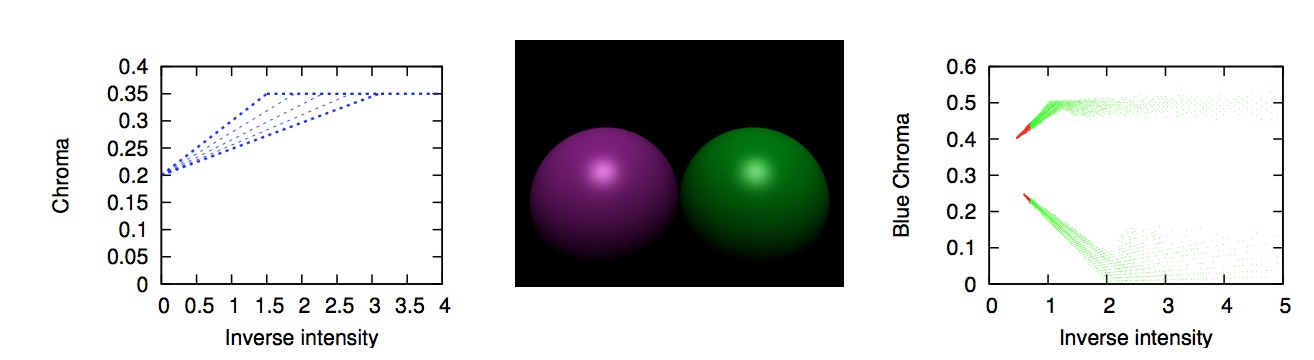
\includegraphics[width=1\textwidth]{iic_space}
    \caption{Pixel distribution in inverse-intensity chromaticity (IIC) space. Left are as ideal distribution, left on a synthetic image (in the center).}
    \label{fig:iic_space}
\end{figure}

The 2D space defined by $\frac{1}{\sum_{i} I_i(x)}$ as domain and $0 \leq \sigma_c \leq 1$ as range is called \emph{inverse-intensity chromaticity (IIC)} space.

An example of the IIC plots for a single channel of a synthetic image are shown in Fig. \ref{fig:iic_space}.
Pixels from the green and purple balls form two clusters. The clusters have spikes that point towards the same location at the $y$-axis. Considering only such spikes from each cluster, the illuminant chromaticity is estimated from the joint $y$-axis intercept of all spikes in IIC space.

Instead of examining the entire pixel distribution, Riess et al.\cite{riess2010scene} perform the analysis over small connected image regions of roughly uniform object color (\emph{superpixels}). Depending on the outcome of our shape analysis, we can either use this local region to obtain an illuminant estimate, or reject it if it does not seem to fulfill the underlying assumptions of the proposed model. Using local regions allows us to incorporate multiple sampling and voting in the estimation of local illuminants.

\section{Human faces splicing detection}

The approach proposed in Chapter 2 is based on two different works, published by Carvalho et al.\cite{carvalho2016illuminant} and Fan et al.\cite{fan2015image}.

The method proposed by Carvalho et al.\cite{carvalho2016illuminant} aims to detect splicing focusing on human faces, minimizing the user interaction. Faces are previously labeled by a human selecting the box within is contained, than the process will associate a label to each face (i.e. \emph{normal} or \emph{fake}).

The method can be divided into four steps:

\begin{enumerate}
\item \emph{Description}: in this step illuminant maps are estimated with the two different approaches, GGE and IIC, and feature vector are generated. Each feature vector is associated with a face pair.
\begin{figure}[h!]
  \centering
    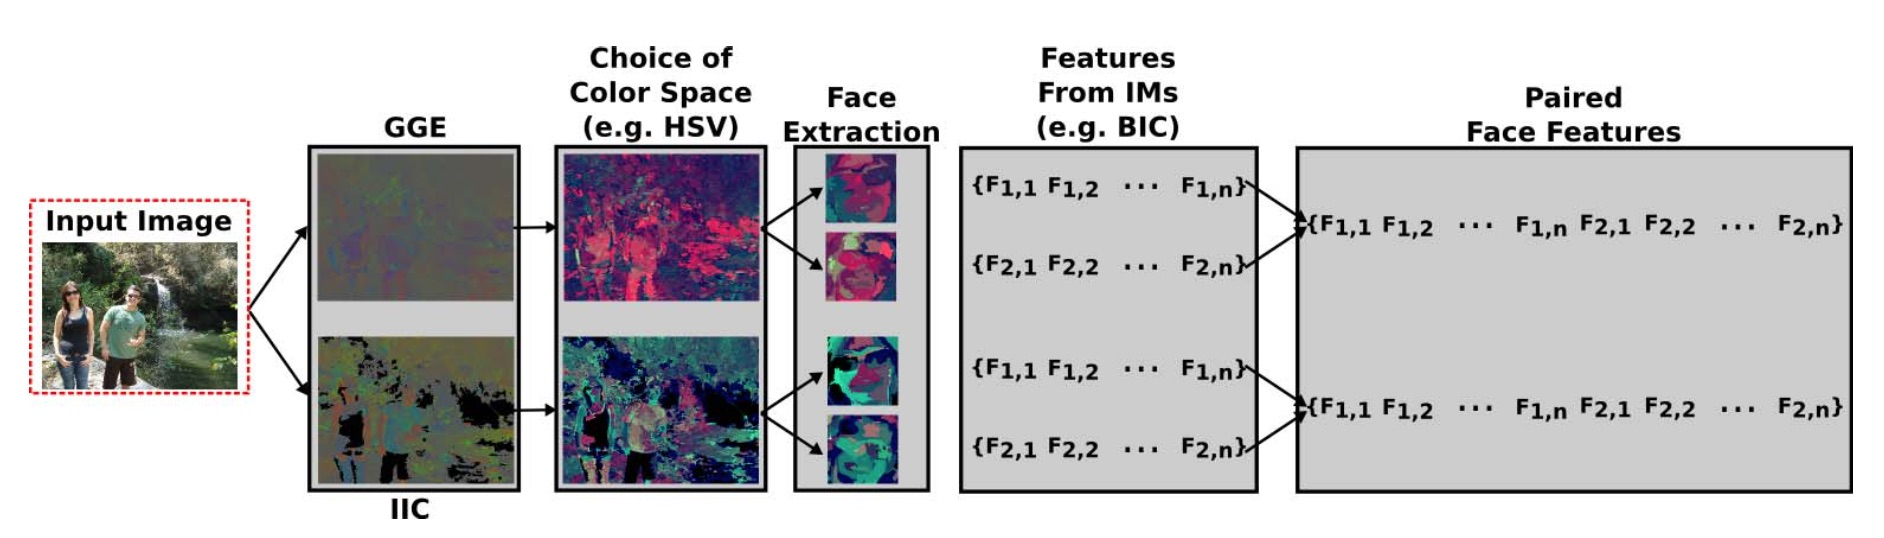
\includegraphics[width=1\textwidth]{tiago_method_extraction}
    \caption{Image description pipeline for extracting paired face feature vectors}
    \label{fig:tiago_method_extraction}
\end{figure}

The Fig. \ref{fig:tiago_method_extraction} shows the image description extraction pipeline. Given an input image, the illuminant maps are estimated and converted to a selected color space (e.g. HSV). So, the faces in the image are extracted (using the defined area). For each face a descriptor is used to generate a feature vector (e.g a color descriptor, texture descriptor or shape descriptors) and finally they are coupled in order to generate paired feature vector simply concatenating the two original vectors.

In this step multiple descriptors and color spaces are used in order to increment the number of final classifiers.

\item \emph{Face Pair Classification}: a set of classification models are trained using the previous step feature vectors. Based on the number of color spaces and descriptors used, a set of KNN classifiers are trained over the paired face feature vectors. The final result is given by a majority voting of all the selected classifiers.

\item \emph{Forgery Classification}: given an image $I$ containing $q$ people (faces), it is characterized by a set $\mathcal{S} = \{\mathcal{P}_1, \ldots, \mathcal{P}_m \}$, where $\mathcal{P}_i$ is the $i$-th paired feature vector and $m = \frac{q(q-1)}{2}, q \geq 2$. If any $\mathcal{P}_i \in \mathcal{S}$ is classified as fake, the image $I$ is classified as fake. Otherwise, the image is considered as pristine.

\item \emph{Forgery Detection}: once knowing that an image is fake, in this stage it is identified which one is more likely to be fake in the image. This is done using a specific SVM classifier.   
\end{enumerate}

\begin{figure}[h!]
  \centering
    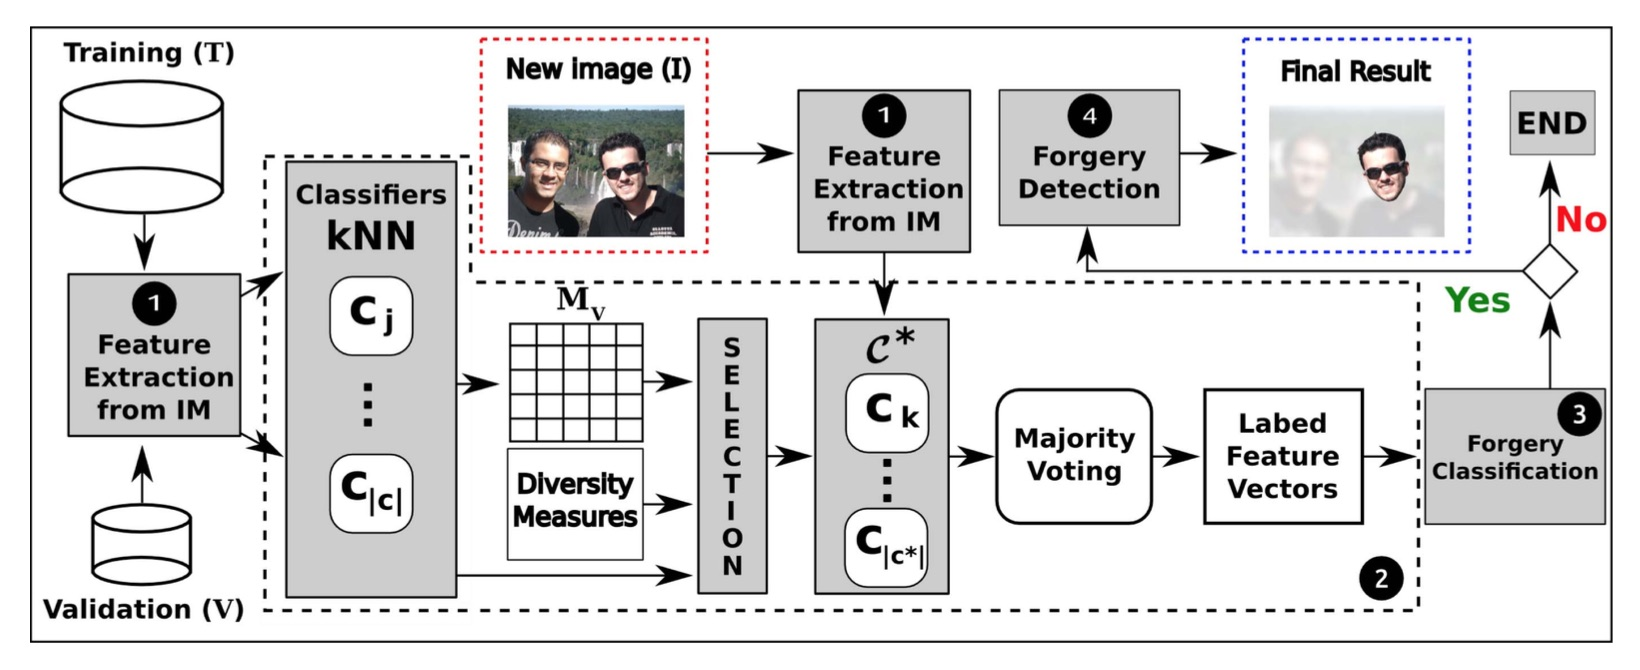
\includegraphics[width=1\textwidth]{tiago_method_full}
    \caption{Image splicing detection over human faces}
    \label{fig:tiago_method_full}
\end{figure}

The Fig. \ref{fig:tiago_method_full} shows the above descripted method pipeline.

\subsection{Method drawbacks}

\section{Region splicing detection}

The other considered approach is based on the work of Fan et al.\cite{fan2015image}. This method relies on the Van de Weijer et al.\cite{van2007edge} Generalized Gray-World framework \ref{eq:ggeframework}. These algorithm perform better on a scene when it is rich of colors, but in a splicing detection scenario we are interest in a specific region of the image.

This approach splits image in vertical and horizontal bands (rectangular regions), assuming that each band contains sufficient colors for a correct illuminant estimation. Five different algorithm are used, deduced from Eq. \ref{eq:ggeframework}: Grey-World, Max-RGB, Shades of Grey, first- order Grey-Edge and second-order Grey-Edge, in order to have as many illuminant estimates for each band.

This algorithm can be divided into two steps:
\begin{enumerate}
\item Subsampling of the image horizontally and vertically
\item Illuminant estimation for each band using the 5 different algorithms and spliced region location.
\end{enumerate}

In the first step the image is sampled into two band categories: horizontal and vertical bands. The height and the width of each band is configured \emph{a priori} based on the minimal height and minimal width separately among the objects of interest. An object of interest is encompassed by a virtual rectangle with its height and width decided by the object itself.

The second step can be also divided into five steps:

\begin{enumerate}
\item For each direction and for each algorithm, a reference illuminant is estimated for a single band.
\item For each direction and for each algorithm, a reference illuminant for each direction is evaluated as the median of all references of that direction. At this stage there are two reference illuminats (one for the vertical and one for the horizontal direction) for each algorithm.
\item A detection map is created, with the same dimensions of the image.
\item For each algorithm, every band estimate are compared with the reference illuminant of that band direction and algorithm with the Euclidean distance. If the distance exceed a fixed threshold, the band is considered fake and all the pixel values in the detection map are increased by one unit.
\item The forgery is located using the resulting thresholded detection map.
\end{enumerate}

\begin{figure}[h!]
  \centering
    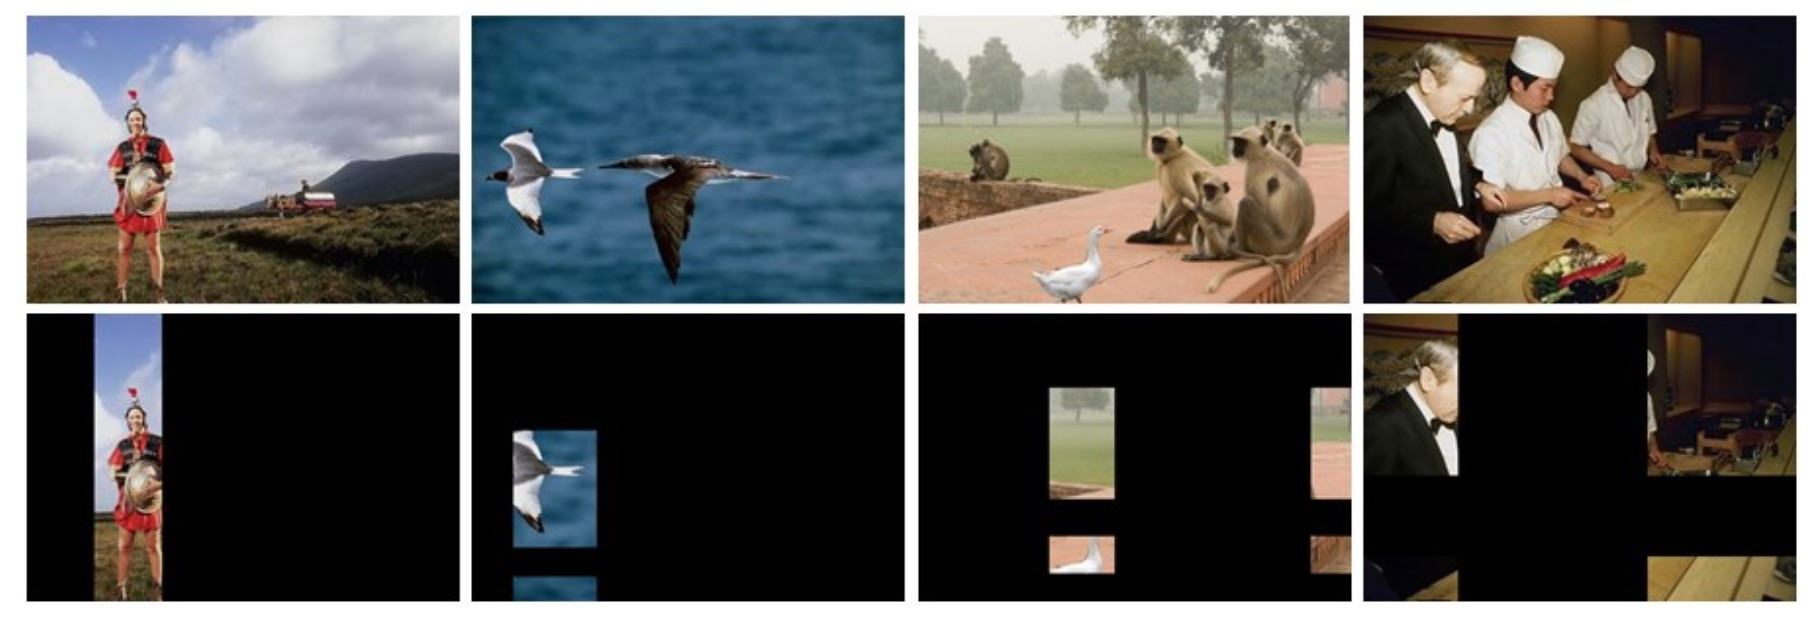
\includegraphics[width=1\textwidth]{regionsmethod}
    \caption{Image regions splicing detection}
    \label{fig:regionsmethod}
\end{figure}

The main advantage of this method is its blind approach: the algorithm is not based on the image content (as it was in the previous case) and no human interaction is needed. The only parameters are the bands minimal dimensions and the threshold. Due these facts it is very simple to implement, but it is also afflicted by false alarm caused by a not easy to tune threshold (which is the key the final step).

\subsection{Method drawbacks}